\def\year{2017}\relax
%File: formatting-instruction.tex
\documentclass[letterpaper]{article} %DO NOT CHANGE THIS
\usepackage{aaai17}  %Required
\usepackage{times}  %Required
\usepackage{helvet}  %Required
\usepackage{courier}  %Required
\usepackage{url}  %Required
\usepackage{graphicx}  %Required
\frenchspacing  %Required

\usepackage{amsmath}
\usepackage{amssymb}
\usepackage{multicol}
\usepackage{algorithmicx}
\usepackage{algorithm}
\usepackage{algpseudocode}
\usepackage{graphicx}

\setlength{\pdfpagewidth}{8.5in}  %Required
\setlength{\pdfpageheight}{11in}  %Required
\setcounter{secnumdepth}{1}



%PDF Info Is Required:
\pdfinfo{
/Title (Cost-Length Tradeoff Heuristics for Bounded-Cost Search)
/Author (Sean Dobson, Patrik Haslum)}

\title{Cost-Length Tradeoff Heuristics for Bounded-Cost Search}
\author{Sean Dobson \\
        University of Auckland \\
        seandobs@gmail.com \\
   \And Patrik Haslum \\
        Australian National University \& CSIRO Data61 \\
        patrik.haslum@anu.edu.au
   }

\begin{document}
\maketitle
\begin{abstract}
Bounded-Cost Search involves solving a planning
problem subject to the constraint that the cost
of the solution must be within a specified cost bound.
We investigate the use of heuristics
to guide a greedy search which solves these kinds of cost bounded planning
problems.
We devise a formulation
which combines heuristic approximations for both solution cost
and solution length. This heuristic adapts previous work in estimating a search node's potential;
the probability that it will lead to a solution within the cost bound.
We also introduce Pareto Front Pattern Databases, which evaluate a number of
pareto optimal solutions in an abstract space to produce
a heuristic which is suited to guiding Bounded-Cost Search.
\end{abstract}
\section{Introduction}
It is well known that classical planning problems can
be solved optimally using heuristic-guided search algorithms such as A* \cite{hart1968formal}.
However, optimal solutions may prove to be too hard to find within the practical
constraints of time and memory. Conversely,
sub-optimal solutions can be found relatively quickly using greedy best-first search.
Historically, work in this area has focused on producing
sub-optimal solutions that are within some factor, \(w\), of the optimum \cite{pohl1970heuristic}.
It is only recently \cite{stern2011potential,thayer2012faster,haslum2013heuristics} that work has been done to consider
the alternative scenario where we are required to produce any sub-optimal solution
as long as its cost is less than or equal to some maximum cost bound, \(C\).
We refer to this as Bounded-Cost Search.

Typically, heuristics for optimal search aim to predict the cost of the optimal solution (eg. PDB heuristics \cite{culberson1996searching,felner2004additive,haslum2007domain,helmert2007flexible}).
These are cheapest-cost heuristics, and they naturally guide the search toward cheaper solutions.
If we weren't concerned with solution cost at all,
then the fastest way to find a solution would be to ignore operator costs completely
and greedily prioritise those nodes which are estimated to be closest to the goal in terms
of the number of actions, i.e. our search should follow a shortest-length heuristic.
However, with Bounded-Cost search, there are different considerations to be
made when designing a heuristic.
We are equally satisfied with any solution within the cost bound,
and this gives us some leeway to sacrifice cost-optimality
and greedily follow shortest-length in order to reduce search time.
But it is clear that we must also take solution cost into account;
greedily following the shortest-length heuristic may actually waste more time
if it chases solutions which exceed the cost bounds.

Our work attempts to strike a balance between these two ideas,
incorporating estimations for both solution length and cost into
a single guiding heuristic which can be used to inform a best-first Bounded-Cost search.
We explore the concepts employed in the development of Potential Search (PTS) \cite{stern2011potential},
which is a best-first search prioritising nodes that are more likely
to lead to a goal within the cost bound.
We show that this can be used to inform a rational tradeoff between the likelihood of finding a solution within the cost bound,
and the time taken to find that solution.
This formulation produces an approximation for the 'expected work'
in finding a solution under a given search node.
Specifically, we estimate the number of nodes that
would need to be expanded on average to find the solution.
We claim that by prioritising our open list by those nodes with the minimum expected work,
the search will minimise the total number of nodes expanded.

Independently of the expected work estimation,
we also produce a modified version of the Pattern Database (PDB) heuristic \cite{culberson1996searching},
which we call the Pareto Front Pattern Database (PFPDB).
In the construction of our PFPDB, a number of cost-length pareto optimal solutions are explored in the abstract space,
allowing our heuristic to produce different values for the same state
depending on how close the node is to the cost bound.
We propose a modified version of Dijkstra's algorithm \cite{dijkstra1959note}, called Pareto Front Dijkstra Search (PFD),
which can be used to efficiently construct the PFPDB.
We also show that techniques for producing additive PDBs \cite{felner2004additive} can also be
applied to PFPDBs, and that we can add together the elements of pareto fronts
to produce a new pareto front of higher quality.

\section{Background}

Past research in the area of bounded-cost search has often involved
either a cost-oriented heuristic \cite{stern2011potential}, a distance-oriented heuristic \cite{haslum2013heuristics},
or some mechanism of alternating between the two \cite{thayer2012faster}.
This research has typically shown the purely distance-oriented heuristics
to be the fastest.

We begin by noting that not all nodes may be extended in to a solution within the cost bound.
Expanding such nodes is obviously a waste of time, and so it would be useful to be able to detect and prune these nodes during our search.
Note the distinction between a state and a search node: a node represents a path to a state in the search space.
With that in mind, suppose that \(n\) is a search node.
We define \(h^*(n)\) to be the cost of the cheapest path from the state represented by \(n\) to the goal,
and we define \(g(n)\) to be the (potentially suboptimal) cost of the path that is represented by \(n\).
Then \(f^*(n) = g(n) + h^*(n)\) is the cost of the cheapest path which extends \(n\) in order to reach the goal.
Clearly, we can extend \(n\)'s path to a solution within the cost bounds if and only if \(f^*(n) \leq C\).
Nodes that don't satisfy this condition should not be expanded by our search, but detecting this would require knowledge of \(h^*(n)\).

\subsection{Potential Search}

Consider that it may be beneficial to repackage an admissible cost-estimating heuristic, \(h\), as a simple pruning function, \(p^C_h\), such that
\[
    p^C_h(n) = 
\begin{cases}
  1,& \text{if } h(n) \leq C - g(n) \\
  0,& \text{otherwise}
\end{cases}
\]
Unfortunately, this discards some of the relevant
information given by \(h\),
but the formulation motivates a further improvement.
In the development of Potential Search (PTS) \cite{stern2011potential},
this idea for a pruning function was augmented to produce real values in the range \([0, 1]\) where
\(p^C(n) = Pr(h^*(n) \leq C - g(n)) \).
So \(p^C\) represents
the probability that \(n\) can be extended to a solution within the cost bound.
PTS refers to \(p^C\) as a node's \textit{potential}.
Strictly speaking, it is true that \(Pr(h^*(n) \leq C - g(n)) \in \{0,1\}\) in a deterministic context,
but for practical purposes we use our heuristic to produce an aggregation of this probability on a per \(h\)-value basis.
Let \(U_h(v)\) give a uniform random distribution over the set of all nodes \(n\) with
\(h(n) = v\).
Then we take \(p^C_h(q, v) = Pr(h^*(n) \leq C - q \mid n \sim U_h(v))\),
such that \(p^C_h(g(n), h(n))\) is the probability that a node \(n'\) randomly chosen
from the set of nodes with \(h(n') = h(n)\) has \(h^*(n') \leq C - g(n)\).

PTS would guide the search by expanding nodes in ascending order of \(\frac{1}{p^C_h(g(n), h(n))}\) (pruning on \(\frac{1}{0} = \infty\)),
and thus direct the search toward nodes which were more likely to lead to a solution within the cost bound.
PTS does not use \(p^C_h\) directly as this function is generally unknown,
but rather it constructs a function \(\phi^C\) that gives approximately the same node ordering of nodes as \(p^C_h\).
Under the assumption that the error \(h^*(n) - h(n)\)
is linear in the size of \(h(n)\),
it has been shown \cite{stern2011potential} that choosing \(\phi^C(g(n), h(n)) = 1 - \frac{h(n)}{C + 1 - g(n)}\)
yields the same ordering as \(p^C_h\). Technically, this formulation is
not explicitly stated in their work.
The standard PTS construction, as given in the paper, takes PTS\(^C(g(n), h(n)) = \frac{h(n)}{C - g(n)}\).
We have chosen to replace \(C\) with \(C + 1\) in our
formulation. This is because when \(h(n) = C - g(n)\), we still want the potential
to be greater than \(0\) in case we have \(h(n) = h^*(n)\).
We have also inverted the term so that \(\phi^C\) more directly
approximates \(p^C_h\), and \(\frac{1}{\phi^C(g(n), h(n))}\) gives the same ordering
as PTS, but with values in the range between \([0, \infty]\) rather than \([0,1]\).

\subsection{BEEPS}
Bounded-Cost Explicit Estimation Potential Search (BEEPS) attempted to improve upon PTS
by incorperating distance-estimating heuristics to guide the search \cite{thayer2012faster}.

Assume that we are given an inadmissible cost heuristic, \(\hat{h}\),
an admissible cost heuristic, \(h\), and an inadmissible distance heuristic \(\hat{d}\).
So it is safe to prune with \(h\), but not with \(\hat{h}\).
At any point during our search, we have a set of nodes, \(open\), which have been generated but are yet to be expanded.
BEEPS takes:
\begin{align*}
        open^C &= \{n \in open : g(n) + h(n) \leq C\} \\
        \widehat{open}^C &= \{n \in open^C : g(n) + \hat{h}(n)\leq C\}
\end{align*}
The BEEPS search strategy then chooses the next node to be expanded with the following rule:
\begin{align*}
    \text{BEEPS}^C(open) = 
\begin{cases}
  \underset{n \in \widehat{open}^C}{\operatorname{argmin\ }} \hat{d}(n), \text{ if } \widehat{open}^C \not = \emptyset \\
  \underset{n \in open^C}{\operatorname{argmax\ }} \phi^C(g(n), \hat{h}(n)), \text{ otherwise}
\end{cases}
\end{align*}
Essentially, BEEPS uses \(\hat{d}\) to guide the search whilst \(\hat{h}\) still reports that a solution
exists within the bounds. Then, when the search runs out of nodes within the inadmissible boundary,
BEEPS reverts to running PTS (with \(\hat{h}\)) on those nodes within the admissible boundary.

\section{A Rational Approach to Combining Cost and Distance Estimations}
Rather than alternating between cost and distance heuristics like BEEPS,
our work attempts to merge them into a single combined heuristic
which rationally accounts for the interaction of these two sources of information.

Consider now that if we had knowledge of the perfect heuristic, \(h^*\),
then \(p^C_{h^*}(g(n), h^*(n)) \in \{0,1\}\) could be computed exactly.
But then, using this in the PTS formulation,
the search would assign every node either \(0\) or \(\infty\),
resulting in a blind search over all nodes with \(f^*(n) \leq C\).
This is obviously not an ideal search strategy,
and it hints at the fact that, beyond simply estimating the potential,
PTS also relies on in its approximation
prioritising nodes with lower \(h\)-values.

Expanding on the ideas of PTS, note that \(\frac{1}{p^C_h(g(n), h(n))}\) is the number of times we expect to have
to draw \(n' \sim U_h(h(n))\) before we find \(n'\) with \(g(n) + h^*(n') \leq C\).
So the expansion of \(n\) is predicated upon the fact that we expect to expand \(\frac{1}{p^C_h(g(n), h(n))}\) other \(n\)-like nodes, along with all of the nodes in their subtrees with \(f\)-levels less than \(C\), before we find a solution within the cost bound.
Then let \(T^C(n)\) predict the size of the \(C\)-bounded subtree rooted at \(n\),
and let \(H^C(n)\) be the expected number of nodes that we will explore before we find the goal
under a node like \(n\):
\[H^C(n) = \frac{T^C(n)}{p^C_h(g(n), h(n))}\]
We will refer \(H^C\) as our \textit{expected work} heuristic.
At each decision point, a rational agent seeking to minimise
the amount of work done in achieving its goal would choose
the alternative which it predicts will minimise the amount of work done in the future.
So rationally speaking, our search strategy should aim to expand the node
which it predicts will result in the fewest number of future node expansions,
which is what the expected work heuristic aims to capture.
Hence, we claim that the search should ideally expand the node which minimises \(H^C(n)\).
With perfect predictions for potential, \(H^C(n)\) would resort to prioritising
nodes with the smallest subtrees, which is ideal for minimising search runtime.

In practice, we don't know \(T^C\) or \(p^C_h\),
but we can approximate \(p^C_h\) with \(\phi^C\),
and \(T^C\) can be estimated.
Let \(b\) denote the average branching factor of the search tree,
and let \(d^C(n)\) give an estimation for the length of the shortest solution from \(n\) to the goal within the cost bound, such that \(d^C(n)^b \approx T^C(n)\).
Then we have:
\[H^C(n) \approx \omega^C(n) = \frac{d^C(n)^b}{\phi^C(g(n), h(n))}\]

Noting that \(\phi^C\) can be a rather poor approximation, in our Future Research section we outline a proposal for approximating \(p^C_h\)
directly via online learning of heuristic errors.

\section{Pareto Front Pattern Databases}

Pattern databases (PDBs) \cite{culberson1996searching} are a commonly used type of heuristic
which solve an abstract version of the problem
in order to provide admissible estimates of the difficulty of
solving the actual problem. Essentially, we construct a 'pattern' abstraction,
which is really just a subset of the variables which make up a state description.
We apply this abstraction to a state by simply removing the variables
which aren't in the pattern.
Likewise, the problem operators are abstracted so that the ignored variables
are stripped from the action preconditions and effects.
This leaves us with a simpler abstract problem,
for which the cost of the cheapest abstract solution gives
an admissible estimate for the cost of the cheapest soluton in the concrete space.
We can perform a backward Dijkstra
search from the goal to find the cheapest path to the goal from
all of the states in the abstract state space. These costs are stored in the pattern database,
to be recalled at a later time during our actual search.
For a given abstraction \(a\), and search node \(n\), we map \(h_a(n) = h^*(a(n))\), which is the cost of the cheapest abstract solution found for \(a(n)\).

We now adapt the PDB methodology to produce a new heuristic for bounded-cost search.
We'll refer to this heuristic as a Pareto Front Pattern Database (PFPDB).
Our idea is simple; for every abstract state in the PFPDB,
we explore all paths from that state to the goal in the abstract space which are \textit{pareto optimal} in their length
and cost. I.e. those solutions for which the length cannot be improved without increasing the cost,
and the cost cannot be improved without increasing the length.
Let \(\succ\) denote the cost-length pareto domination relation
such that for two paths \(\pi\) and \(\pi'\), we have:
\begin{align*}
  \pi \succ \pi' \iff &length(\pi) \leq length(\pi') \land \\
  &cost(\pi) \leq cost(\pi') \land \\
  &(length(\pi) < length(\pi') \lor \\
  &cost(\pi) < cost(\pi'))
\end{align*}
(Note that \(\pi \succ \pi'\) means \(\pi\) dominates, i.e., is strictly
better than, \(\pi'\).)
Supposing that \(\Pi(s)\) gives the set of all paths from  a state \(s\) to the goal,
we define a state \(s\)'s \textit{pareto front} as the subset of paths in \(\Pi(s)\) which are pareto optimal:
\[
  \Pi^*(s) = \{\pi \in \Pi(s) : \lnot \exists \pi' \in \Pi(s), \pi' \succ \pi\}
\]
For a given abstraction \(a\),
our PFPDB heuristic finds \(\Pi^*(s_a)\)
for each abstract state, \(s_a\), reachable from the abstracted goal.
Then with every pareto optimal abstract solution \(\pi \in \Pi^*(s_a)\),
we store the corresponding \textit{pareto pair}, \((cost(\pi), length(\pi))\),
in our database.
Then we can easily implement a function \(\Pi_{a}(n) =  \Pi^*(a(n))\)
mapping concrete search nodes to their pre-computed abstract pareto fronts.

These pareto fronts may be used in various ways to compute the heuristic value.
E.g. we could return the length of the shortest abstract solution within the cost bounds:
\begin{align*}
  \Pi^C_a(n) = \{ \pi \in \Pi_a(n) : g(n) + cost(\pi) \leq C\} \\
  d^C_a(n) =
  \begin{cases}
  \underset{\pi \in \Pi^C_a(n) }{\operatorname{min\ }} length(\pi) ,& \text{if } \Pi^C_a(n) \not = \emptyset \\
    \infty ,& \text{otherwise}
  \end{cases}
\end{align*}
(pruning on \(d^C_a(n) = \infty\)).
We could also substitute the lengths and costs into formula for \(\omega^C(n)\)
as the values for \(d(n)\) and \(h(n)\) respectively:
\begin{align*}
  \omega^C_a(n) =
  \begin{cases}
  \underset{\pi \in \Pi^C_a(n) }{\operatorname{min\ }} \frac{length(\pi)^b}{\phi^C(g(n), cost(\pi))} ,& \text{if } \Pi^C_a(n) \not = \emptyset \\
    \infty ,& \text{otherwise}
  \end{cases}
\end{align*}
In general, this could be posed as the minimisation of some objective function, \(O(n, \pi)\),
over all \(\pi \in \Pi^C_a(n)\).

\subsection{Computing the Pareto Fronts Efficiently}

We now briefly describe an algorithm which
will find the pareto fronts for every node reachable
via a regression from the goal. Extending
the standard PDB approach, we use a modified
version of Dijkstra's \shortcite{dijkstra1959note} algorithm.
Pareto Front Dijkstra's Search (PFD) is different from
the ordinary Dijkstra's algorithm in two respects.
Firstly, PFD expands nodes in lexicographical order of cost and then length.
And secondly, when considering a node \(n\) for expansion,
which represents a path from some state \(s\) to the goal,
we only expand \(n\) if that path is nondominated in terms of cost and length
by any of the previously expanded paths to \(s\).
If \(n\) is expanded, then \((h(n), d(n))\) is recorded in
the pareto front for \(s\).

We claim that PFD has the following property:
\textit{PFD terminates after having explored precisely those nodes
  which represent pareto optimal paths to the goal.} \\
\textbf{Proof:}
Note that our search proceeds backward from the goal, so for a search node \(n\)
which represents a path from \(n\)'s state to the goal, we let \(h(n)\) and \(d(n)\)
represent the respective cost and length of that path.
Now observe that all of the subpaths of any pareto optimal path must they themselves
be pareto optimal. Otherwise, we could swap that sub-optimal subpath out for
one that dominates it and produce a new solution which dominates the original one, contradicting our premise
that that path was pareto optimal.
Assume now that we had expanded precisely those pareto optimal nodes with \(h(n) \leq i\).
Then the pareto optimal nodes with \(h(n) = i + 1\) could be found in the open list
as children of their pareto optimal parents.
If \(n\) and \(n'\) represent different paths to the same state,
then \(n' \succ n\) iff \(h(n) \geq h(n')\) and \(d(n) \geq d(n')\)
and at least one of those inequalities is strict.
But by our lexicographical ordering and by our assumption,
when we consider \(n\) for expansion,
all pareto optimal nodes which could dominate \(n\) must have been found already.
And so it is sufficient to determine \(n\)'s pareto optimality by only checking
that it is not dominated by any of the previously explored pareto optimal nodes for that state.
So, of the nodes with \(h(n) = i + 1\), PFD will expand exactly those nodes which
are pareto optimal. By induction from a base case of the goal node \(G\) having \(h(G) = d(G) = 0\), which is obviously
pareto optimal, PFD expands precisely the set of pareto optimal nodes. QED

As a minor improvement to PFD,
we can use a slightly stricter pre-requisite for node
expansion which requires that the node is not only pareto optimal,
but it also has a unique cost and length when compared with
the pareto optimal solutions already in the PFPDB.
This essentially removes duplicate entries from our list of pareto pairs.
We also note that the most recent pareto optimal pair added to the list for a state
is both the most expensive and shortest pareto optimal solution found so far for that state.
Then the expansion check can be made for a node \(n\) in \(O(1)\)
by simply taking the last entry in the list of pareto pairs for \(n\)'s state,
\((h_{max}, d_{min})\), and checking that \(d(n) < d_{min}\).
As another simple way of speeding up PFD, if we know that
none of the pareto pairs exceeding \(cost(\pi) > C\) will be used
to produce the final heuristic value,
then we can prune those nodes with \(h(n) > C\) from our abstract search.

\subsection{Additive Pareto Front Pattern Databases}

Some techniques for improving PDB heurstics
involve the generation of a set of abstractions
over which the PDB values can be summed together
in order to produce an admissible heuristic value \cite{felner2004additive}.
We say that such a set of patterns is \textit{additive}.
We can take advantage of this kind of additivity in our work
by adding together the pareto fronts.
Pareto pairs are added together by summing their costs and lengths:
\begin{align*}
  cost(\pi_1 + \pi_2) &=\ cost(\pi_1) + cost(\pi_2)\\
  length(\pi_1 + \pi_2) &=\ length(\pi_1) + length(\pi_2)
\end{align*}
Lists of pareto pairs are added together by
taking the pairwise sums of every combination of pareto pairs:
\[\Pi_1 + \Pi_2 = \bigcup_{(\pi_1, \pi_2) \in \Pi_1 \times \Pi_2} \pi_1 + \pi_2 \]
Note that not all members of \(\Pi_1 + \Pi_2\) are guaranteed to be
pareto optimal. Taking the subset of pareto optimal pairs,
we obtain:
\begin{align*}
  \Pi_1 +^* \Pi_2 = \{\pi \in \Pi_1 + \Pi_2 :\ &\lnot \exists \pi' \in \Pi_1 + \Pi_2, \\
 &\pi' \succ \pi\}
\end{align*}
Careful consideration must be made as to the implementation of this operation;
this could be a bottleneck in the time taken to compute the final heuristic value.
With that in mind, we have devised the following two alternative approaches:
\begin{enumerate}
\item
  We can use the same technique applied in PFD
  to find \(\Pi_1 +^* \Pi_2\) via a single pass
  over the lexicographically sorted \(\Pi_1 + \Pi_2\).
  If \(n = |\Pi_1|, m = |\Pi_2|\), then sorting takes \(O(n m \cdot log(n m))\),
  for the \(n m\) pairs in \(\Pi_1 + \Pi_2\).
  Checking for pareto optimality and appending to the new pareto front takes \(O(1)\) per pair,
  so sorting dominates the complexity.
\item
  Our second approach will compute the minimum \(cost\)-value associated with every \(length\)-value.
  Let
  \begin{align*}
  length_{min} &= \underset{\pi \in \Pi_1 + \Pi_2}{\operatorname{min\ }} length(\pi) \\
  length_{max} &= \underset{\pi \in \Pi_1 + \Pi_2}{\operatorname{max\ }} length(\pi) \\
  \delta &= length_{max} - length_{min}
  \end{align*}
  We note that with a single iteration over \(\Pi_1 + \Pi_2\),
  we can easily construct an array of size \(\delta\) that maps
  \begin{align*}
    cost_{min}[d] &= \underset{\pi \in \Pi_1 + \Pi_2}{\operatorname{min\ }} cost(\pi) \\
    &\text{s.t. } length(\pi) = d + length_{min}
  \end{align*}
  (with \(cost_{min}[d] = \infty\) if no such \(\pi\) exists).
  Then we can iterate over this map in ascending order of possible \(length\)-values,
  \(d  = 0, \ldots, \delta\), inserting \[(cost_{min}[d], d + length_{min})\] into the pareto front if
  we have \(cost_{min}[d] \not = \infty \land cost_{min}[d] < \underset{d' < d}{\operatorname{min\ }} cost_{min}[d']\).
  Every inserted pair is pareto optimal because there is no
  \(\pi \in \Pi_1 + \Pi_2\) for which \(length(\pi) < d + length_{min}\)
  and \(cost(\pi) \leq cost_{min}[d]\).
  Tracking the value of \(\underset{d' < d}{\operatorname{min\ }} cost_{min}[d']\) as we go
  yields a complexity of \(O(\delta)\) for this iteration.
  Then we have a combined complexity of \(O(nm + \delta)\) for both stages of the computation.
  
\end{enumerate}
Observe that in bounded cost search,
the cost bound can be used to limit the size of the pareto fronts
by pruning those pairs with \(cost(\pi) > C\).
No two pairs in a front may have the same cost (assuming PFD removes duplicates),
and so \(n,m \leq C\).
We can do this same pruning when constructing the summed pareto front;
our implementation cuts the enumeration of \(\Pi_1 + \Pi_2\) short so as to exclude all pairs with \(cost(\pi) > C\).
In domains with large actions costs, it will likely be the case that \(nm << C^2\),
particularly because path cost and length are positively correlated in the presence of
positive action costs.
Under the assumption that \(\delta\) would be relatively small for most of the evaluated
pareto fronts (i.e. \(\delta < C\)), we went with the \textbf{second approach} in our final implementation.

For multiple additive abstractions,
we can simply apply the \(+^*\)
operation repeatedly to sum them all together.
If \(\Xi = \{\Pi_{1}, \Pi_{2}, \ldots\}\) is a set of additive PFPDBs,
and \(n\) is a search node, then (with some abuse of notation)
we take:
\begin{align*}
\Xi(n) &= \underset{\Pi_{i} \in \Xi}{{\sum}^*} \Pi_{i}(n) \\
&= \Pi_{1}(n) +^* (\Pi_{2}(n) +^* (\ldots)) \\
\Xi^C(n) &= \{\pi \in \Xi(n) : g(n) + cost(\pi) \leq C\}
\end{align*}
In our implementation, we compute \(\Xi^C(n)\) directly
by bounding each \(+^*\) operation by the relative cost bound \(C - g(n)\).

\subsection{Canonical Pareto Front Pattern Databases}

Some techniques for finding sets of additive PDBs will
produce a Canonical PDB, which is set of sets of additive PDBs \cite{haslum2007domain}.
For a given state, within each additive set of PDBs, the \(h\)-values for that state are summed.
Then the final heuristic value is given by maxing over those summed totals.
Each summed total is admissible, and so the max is admissible.
Note that, other than for pruning out-of-bounds nodes, admissibility is not an important requirement for guiding our bounded-cost search.
As long as our CPDB returns \(\infty\) when any of
the additively summed \(h\)-values exceeds \(C - g(n)\),
we are free to return an inadmissible heuristic value.
Suppose, then, that our PDB records both the cost and length of the cheapest-cost path as a pareto pair.
For each set of additive PDBs, our CPDB would compute an admissibly summed pair
by adding the additive costs and lengths together, pruning if any summed cost exceeds \(C - g(n)\).
We propose that the CPDB be parameterised with an objective function of the form \(O(n, \pi)\) which
measures the objective value of a summed pareto pair \(\pi\) with respect to the search node \(n\).
We also parameterise our CPDB with an aggregator function
that replaces the max aggregation (e.g. we might sum the objective values rather than max over them).
Then our heuristic returns the aggregation of each summed pair's objective value.

Now we extend these ideas to PFPDBs, in which we are given not only the cheapest-cost pair, but the entire pareto front of pairs.
This gives rise to the notion of a Canonical Pareto Front Pattern Database (CPFPDB).
For each set of additive PFPDBs in the CPFPDB, we find the additively summed pareto front given by the \(\sum^*\) operation (bounded by \(C - g(n)\)).
If that additively summed pareto front is empty (because the additive sum of the cheapest solutions still exceeded the cost bound), then we prune the node.
Otherwise, with that summed pareto front,
we first \textit{minimise} the objective function over each of the pareto pairs,
producing a single minimum objective value for each set of additive PDBs.
Then we apply the aggregator to these minimum objective values (just like with CPDBs), giving us our heuristic value.

For a cost bound \(C\), and aggregator \(A\), and an objective function \(O\), we notate these parameterisations with CPDB\(^C[A \text{ } O]\) and CPFPDB\(^C[A \text{ } O]\).
If we are given a CPFPDB \(\Psi\), and a node \(n\),
then for each set of additive PFPDBs \(\Xi_i \in \Psi\), we compute:
\begin{align*}
\Xi_i(n) &= \underset{\Pi_{j} \in \Xi_i}{{\sum}^*} \Pi_{j}(n) \\
\Xi^C_i(n) &= \{\pi \in \Xi_i(n) : g(n) + cost(\pi) \leq C)\} \\
v^C_i &=  
\begin{cases}
  \underset{\pi \in \Xi^C_i(n)}{\operatorname{min\ }} O(n, \pi),& \text{if } \Xi^C_i(n) \not = \emptyset \\
  \infty, & \text{otherwise}
\end{cases}
\end{align*}
  And finally, our heuristic returns:
\[\Psi^C[A \text{ } O](n) = A(v^C_1, v^C_2, \ldots)\]
With \(A\) returning \(\infty\) if any \(v^C_i = \infty\) (meaning that the \(n\) gets pruned).

If \(\Psi\) were a CPDB instead, then the only difference is that
\(\Pi_{j}(n)\) would be a singleton set containing the cheapest-cost pareto pair.

\section{Experiments}

We tested the effectiveness of the PFPDB heuristic in
a bounded-cost greedy search on the problems
from the satisficing track of the IPC6, 2008
International Planning Competition.
The results of the competition were used to set cost bounds for our experiment.
For each problem, two cost bounds were tested:
\begin{itemize}
\item
  The cost of the second best plan for that problem found by any of the planners that
  participated in IPC6, minus 1.
\item
  The cost of the best plan from IPC6.
\end{itemize}
Each problem is run with a 1GB memory limit and a
time limit of 10 minutes.
Upon the termination of each planner instance,
we recorded whether the problem was solved, if the planner ran
out of memory, or if it ran out of time.

We use the iPDB hill climbing method \cite{haslum2007domain}
to generate our set of patterns.
Our heuristic was implemented by modifying the Fast Downward planner
implementation for iPDBs.
Firstly, we altered the Dijkstra searches so that
they were constrained to not expand any abstract nodes with \(h^*(n_a) > C\),
and for each node expanded we store the length as well as cost.
Secondly, we generalised the iPDB heuristic computation
to allow for user-specified aggregator and objective functions.
And finally, we added an optional extra step to the iPDB construction
which runs PFD search (also bounded by \(C\)) on each of the pattern abstractions
in order to generate the set of PFPDBs.
The heuristics without the PFD search will be labeled
as iPDB\(^C\), whereas those that did do the PFD search are labeled as iPFPDB\(^C\).
All instances of the hill-climbing were
run with a max hill-climbing time of 120 seconds, a cost bound,
and with all other parameters set to the default iPDB settings for Fast Downward.
The aggregator functions that we tested were \(\max\) and \(\sum\).
We tested the following objective functions:
\begin{itemize}
\item
  \(h(n, \pi) = cost(\pi)\)
\item
  \(d(n, \pi) = length(\pi)\)
\item
  \(\frac{1}{\phi^C}(n, \pi) = \frac{1}{\phi^C(g(n), cost(\pi))} = 1 / (1 - \frac{cost(\pi)}{C+1 - g(n)}\))
\item
  \(\omega^C(n, \pi) = \frac{length(\pi)^b}{\phi^C(g(n), cost(\pi))}\)\\
  Where \(b\) is the average branching factor for the search tree
  at the time of \(n\)'s evaluation. If \(u\) is
  the depth of the deepest node evaluated by the heuristic, and \(T_{u-1}\) is
  the number of nodes evaluated up to depth \(u-1\),
  we take \[b =
  \begin{cases}
    \sqrt[u-1]{T_{u-1}} ,& \text{if } T_{u-1} >= 10000 \\
    1 ,& \text{otherwise}
  \end{cases}
  \]
\end{itemize}
Note that, because we constrain the summed pareto front by \(C\),
none of the evaluated pareto pairs will have \(g(n) + cost(\pi) > C\).
This means that the \(d\) objective finds length of the shortest pareto optimal abstract solution
within the cost bound, and \(\phi^C\) won't return a negative value.

The combinations of cost bound, i(PF)PDB, aggregator, and objective that we tested are shown in Tables \ref{tab:resultsBest} and \ref{tab:resultsSecondBest}.
FF\(^C[d]\) is our label for the unit-cost FF heuristic which has been shown 
to perform extremely well in bounded cost search \cite{haslum2013heuristics}.
With FF guiding the greedy search,
we used iPDB\(^C[\max h]\) to admissibly prune nodes exceeding the cost bound.
We also tested A* with the ordinary iPDB (labeled \(g + \) iPDB\(^C[\max{h}]\)).
The only iPFPDB objectives that we tested were \(d\) and \(\omega^C\)
because both \(\frac{1}{\phi^C}\) and \(h\) are always
minimised by the cheapest pareto pair (so iPDB and iPFPDB would return
the same value).

\section{Results}

\begin{table*}
\caption{No. of Problems Solved / Ran out of memory / Ran out of time,
with \(C =\) the cost of the \textbf{CHEAPEST} IPC6 plan.}
\label{tab:resultsBest}
\begin{tabular}{| l | l | l | l | l | l |}
\hline
             & FF\(^C[d]\)      & \(g + \) iPDB\(^C[\max{h}]\)    & iPDB\(^C[\sum{h}]\) &  iPDB\(^C[\max \frac{1}{\phi^C}]\) & iPDB\(^C[\sum \frac{1}{\phi^C}]\) \\
\hline
Elevators    & 13 / 0 / 17    & 2 / 12 / 16     & 2 / 15 / 13     & 2 / 12 / 16       & 4 / 10 / 16 \\
Openstacks   & 24 / 0 / 6     & 12 / 18 / 0     & 12 / 18 / 0     & 12 / 18 / 0       & 12 / 18 / 0 \\
Parcprinter  & 21 / 0 / 9     & 15 / 3 / 12     & 26 / 1 / 3      & 16 / 2 / 12       & 20 / 3 / 7  \\
Pegsol       & 24 / 0 / 6     & 20 / 0 / 10     & 22 / 0 / 8      & 22 / 0 / 8        & 22 / 0 / 8  \\
Scanalyzer   & 18 / 5 / 7     & 11 / 19 / 0     & 21 / 9 / 0      & 12 / 18 / 0       & 12 / 18 / 0  \\ 
Sokoban      & 28 / 0 / 2     & 24 / 6 / 0      & 27 / 3 / 0      & 25 / 5 / 0        & 25 / 5 / 0  \\
Transport    & 8 / 0 / 22     & 6 / 17 / 7      & 28 / 1 / 1      & 6 / 19 / 5        & 7 / 18 / 5   \\ 
Woodworking  & 6 / 18 / 6     & 6 / 18 / 6      & 8 / 18 / 4      & 6 / 18 / 6        & 6 / 18 / 6  \\
\hline
total        & 142 / 23 / 75  & 96 / 93 / 51    & 146/65/29   & 101/92/47     & 108 / 90 / 42  \\
\hline
\end{tabular}

\begin{tabular}{| l | l | l | l | l |}
\hline
             & iPDB\(^C[\sum d]\)  & iPDB\(^C[\sum \omega^C]\)  & iPFPDB\(^C[\sum d]\)  &  iPFPDB\(^C[\sum \omega^C]\)\\
\hline
Elevators    & 15 / 9 / 6        & 19 / 8 / 3        & 18 / 8 / 4          & 17 / 8 / 5 \\
Openstacks   & 24 / 6 / 0        & 24 / 6 / 0        & 24 / 6 / 0          & 24 / 6 / 0 \\
Parcprinter  & 24 / 1 / 5        & 18 / 2 / 10       & 24 / 1 / 5          & 18 / 2 / 10 \\
Pegsol       & 24 / 0 / 6        & 24 / 0 / 6        & 24 / 0 / 6          & 24 / 0 / 6 \\
Scanalyzer   & 23 / 7 / 0        & 23 / 7 / 0        & 23 / 7 / 0          & 23 / 7 / 0 \\ 
Sokoban      & 27 / 3 / 0        & 27 / 3 / 0        & 27 / 3 / 0          & 27 / 3 / 0 \\
Transport    & 27 / 2 / 1        & 27 / 1 / 2        & 28 / 1 / 1          & 27 / 1 / 2 \\ 
Woodworking  & 6 / 18 / 6        & 7 / 18 / 5        & 6 / 18 / 6          & 7 / 18 / 5 \\
\hline
total        & 170 / 46 / 24     & 169 / 45 / 26     & 174 / 44 / 22       & 167 / 45 / 28 \\
\hline
\end{tabular}

\end{table*}

\begin{table*}
\caption{No. of Problems Solved / Ran out of memory / Ran out of time,
with \(C =\) the cost of the \textbf{2nd CHEAPEST - 1} IPC6 plan.}
\label{tab:resultsSecondBest}
\begin{tabular}{| l | l | l | l | l | l |}
\hline
             & FF\(^C[d]\)      & \(g + \) iPDB\(^C[\max{h}]\)    & iPDB\(^C[\sum{h}]\) &  iPDB\(^C[\max \frac{1}{\phi^C}]\) & iPDB\(^C[\sum \frac{1}{\phi^C}]\) \\
\hline
Elevators    & 23 / 0 / 7     & 2 / 12 / 16     & 2 / 14 / 14     & 2 / 12 / 16       & 4 / 10 / 16        \\
Openstacks   & 24 / 0 / 6     & 12 / 18 / 0     & 12 / 18 / 0     & 12 / 18 / 0       & 12 / 18 / 0       \\
Parcprinter  & 20 / 0 / 10    & 15 / 3 / 12     & 26 / 1 / 3      & 20 / 1 / 9        & 24 / 1 / 5         \\
Pegsol       & 25 / 0 / 5     & 20 / 0 / 10     & 22 / 0 / 8      & 22 / 0 / 8        & 22 / 0 / 8        \\
Scanalyzer   & 19 / 5 / 6     & 11 / 19 / 0     & 21 / 9 / 0      & 12 / 18 / 0       & 12 / 18 / 0       \\ 
Sokoban      & 28 / 0 / 2     & 24 / 6 / 0      & 27 / 3 / 0      & 22 / 8 / 0        & 22 / 8 / 0        \\
Transport    & 8 / 0 / 22     & 6 / 17 / 7      & 29 / 0 / 1      & 6 / 19 / 5        & 6 / 19 / 5        \\ 
Woodworking  & 6 / 18 / 6     & 6 / 18 / 6      & 9 / 18 / 3      & 6 / 18 / 6        & 7 / 18 / 5        \\
\hline
total        & 153 / 23 / 64  & 96 / 93 / 51    & 148 / 63 / 29   & 102 / 94 / 44     & 109 / 92 / 39     \\
\hline
\end{tabular}

\begin{tabular}{| l | l | l | l | l |}
\hline
             & iPDB\(^C[\sum d]\)  & iPDB\(^C[\sum \omega^C]\)  & iPFPDB\(^C[\sum d]\)  &  iPFPDB\(^C[\sum \omega^C]\)\\
\hline
Elevators    & 22 / 7 / 1      & 25 / 5 / 0          & 23 / 6 / 1        & 26 / 3 / 1 \\
Openstacks   & 24 / 6 / 0      & 24 / 6 / 0          & 24 / 6 / 0        & 24 / 6 / 0 \\
Parcprinter  & 24 / 1 / 5      & 25 / 1 / 4          & 24 / 1 / 5        & 25 / 1 / 4 \\
Pegsol       & 24 / 0 / 6      & 24 / 0 / 6          & 24 / 0 / 6        & 24 / 0 / 6 \\
Scanalyzer   & 22 / 8 / 0      & 23 / 7 / 0          & 22 / 8 / 0        & 23 / 7 / 0 \\
Sokoban      & 27 / 2 / 1      & 27 / 2 / 1          & 27 / 2 / 1        & 27 / 2 / 1 \\
Transport    & 29 / 0 / 1      & 29 / 0 / 1          & 29 / 0 / 1        & 29 / 0 / 1 \\
Woodworking  & 6 / 18 / 6      & 9 / 18 / 3          & 7 / 18 / 5        & 9 / 18 / 3 \\
\hline
Total        & 178 / 42 / 20   & 186 / 39 / 15       & 180 / 41 / 19     & 187 / 37 / 16 \\
\hline
\end{tabular}

\end{table*}

\begin{figure*}
\centering
\caption{iPDB\(^C[\sum \omega^C]\) vs. iPFPDB\(^C[\sum \omega^C]\) node evaluation statistics for the \textbf{CHEAPEST} cost bounds}
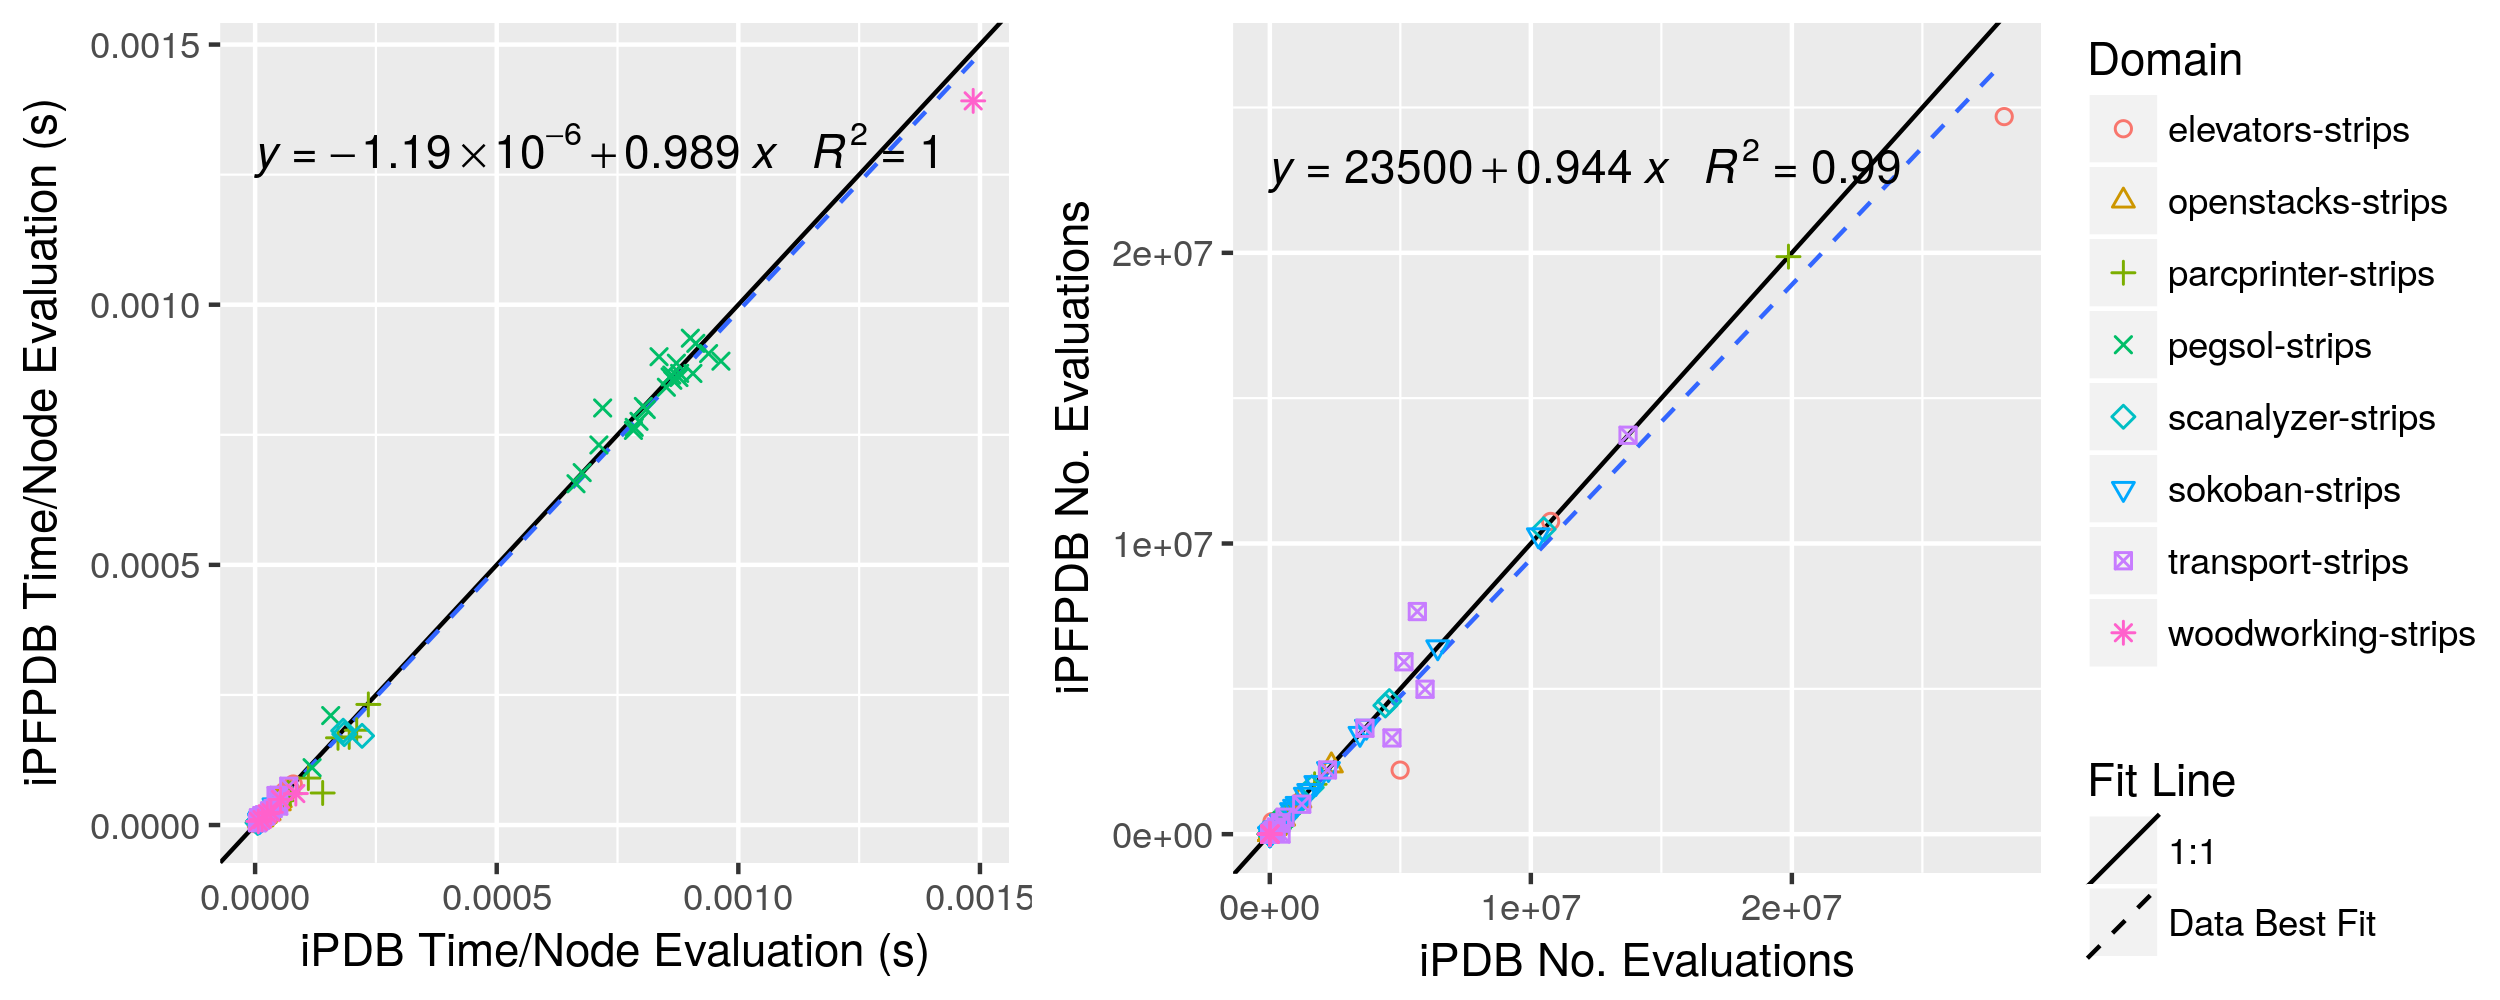
\includegraphics[width=17cm]{pernodeevals}
\label{fig:tpnevals}
\end{figure*}

Results for the experiment are shown in Table \ref{tab:resultsBest} (cheapest) and Table \ref{tab:resultsSecondBest} (2nd cheapest - 1).
Prior to exploring these results, we will note that
in the 'Woodworking' domain, the majority of the problems
caused the iPDB and iPFPDB heuristics to run out of memory
during the iPDB hill climbing. So those results are not particularly interesting
beyond the observation that the iPDB heuristic is not suited to some specific domains.

It appears that the differences between iPDB and iPFPDB were negligible
in terms of the number of problems solved.
iPFPDB performs slightly better with loose bounds,
but under the tight bounds the iPFPDB\(^C[\sum \omega^C]\) heuristic actually did a little bit worse
than iPDB (in the Elevators domain).
This is perhaps a result of the fact that, under tight cost-bounds,
the search will end up needing to find cheaper solutions.
So assigning nodes an heuristic value derived from cost-suboptimal paths may end up
being overly optimistic.
However, even with tight bounds, the \(d\) objective did show some improvement when using the PFPDB implementation.
We must also consider the fact that pareto front
summation introduces a slow-down to the heuristic evaluation that is otherwise not present in the ordinary iPDB computation.
In testing this, we compared the time per node evaluation, and the total number of nodes evaluated, for iPDB\(^C[\sum \omega^C]\) and iPFPDB\(^C[\sum \omega^C]\), when using the tighter bounds.
These results are shown in Figure \ref{fig:tpnevals}.
They showed that both heuristics perform nearly identically in terms of per-node evaluation time
and number of nodes evaluated.
These observations would be explained if
the pareto fronts being generated by the PFD searches were mostly
just a singleton set, with the cheapest and shortest path being identical.
Perhaps the domains that we tested were not 'solution-rich' in their abstracted
spaces, or perhaps the correlation between path length and cost
was so significant that, even if there were multiple paths to the abstract states,
very few of them were pareto optimal.
Either way, this would need to be tested with a more
in-depth experiment.

In terms of the best objective function,
the results suggest that iPDB/iPFPDB with the \(d\) and \(\omega^C\) objectives
produce the best results, with \(d\) performing slightly better under the tight cost bound,
and \(\omega^C\) performing better under the loose cost bound.
The \(d\) objective far outperformed the \(h\) objective, which
confirms that distance-oriented heuristics
perform better than cost-oriented ones in bounded-cost search.
The fact that \(\omega^C\) did worse than \(d\) under the tight cost bounds
is evidence against our conjecture that \(\omega^C\) is always the rational
choice when it comes to bounded-cost search. It does, however, show that
the idea has some merit. It should be noted that,
in cases where the cheapest solution found by any IPC6 planner
was also the optimal solution, our search can only find that solution
by expanding a node right on the cost-boundary. \(\omega^C\) penalises
these nodes quite heavily, but it would make more sense to prioritise the
exploration of nodes on the boundary, given that we know that a solution exists there.
We may also excuse some
of this poor performance as a result of the low quality potential
approximations given by \(\phi^C\) and
our estimate for the branching factor \(b\).
This has motivated us to devise better methods for predicting potential,
which we describe in the Future Research section at the end of this paper.
Likewise, better approximations for the subtree size may also improve the expected
work estimates.

Of the iPDB settings that we tested, iPDB\(^C[\max \frac{1}{\phi^C}]\) performed the worst,
which is in line with previous results testing the quality of the PTS heuristic \cite{haslum2013heuristics}.
That work conjectures that this is due to the failure of the linear-error
assumption, but we offer an alternative explanation.
We claim that the poor performance of PTS comes from the fact that it is
not the correct measure if we seek to find a bounded solution \textit{quickly}.
PTS follows those nodes which are most likely to lead to a bounded solution,
but it makes no considerations as to how long that solution will take to find.
The PTS strategy may work best in minimising the number of out-of-bounds nodes
which are generated, but it ignores nodes
which may be simultaneously close to the bound (high risk) and close to the goal (high reward).
This is somewhat supported by the fact that the \(\omega^C\) and \(d\) heuristics outperform
\(\frac{1}{\phi^C}\) by a wide margin,
as these heuristics prioritise nodes for which reaching
the goal will take the least amount of work.

iPDB\(^C[\sum \frac{1}{\phi^C}]\) solved more problems than the iPDB\(^C[\max \frac{1}{\phi^C}]\) version.
This may be because the \(\sum\) version introduces a larger distinction
in node priorities by incorperating more PDB values and extending the integer range over which the final heuristic values are produced. Hence our eager search can prioritise nodes
for which all of the PDBs yielded consistently low \(\frac{1}{\phi^C}\) values, rather than
just a low maximum. This also justifies our decision
to use the \(\sum\) aggregator on all of the other greedy PDB heuristics.
As an aside, note that \(\sum\) gives the same ordering as
taking a floating point arithmetic mean of the objective values,
because the same number of objective values are aggregated every time.
Fast Downward does not support floating point node priorities, so \(\sum\)
made more sense in our implementation.

Unsurprisingly, it seems that tighter cost bounds generally reduce the number of problems solved by our heuristics,
to varying degrees. A* and \(h\) weren't affected much,
which was to be expected because if a node's \(f\)-level is within the cost bound,
then these objectives produce the same heuristic value regardless of what that cost bound actually is.
Likewise, the two versions of PTS don't seem to be particularly influenced
by the tighter cost bound. This may have been caused by there being
too little difference in the two cost bounds tested,
but the fact that \(\omega^C\) (and to a lesser extent, \(d\))
showed significant differences in performance suggests otherwise.
It may be the case that \(\omega^C\) and \(d\) are better
at taking advantage of the loose cost bounds to find solutions
quickly. These objectives essentially behave like a greedy search
on shortest-path when the cost bounds are loose.

In considering why iPDB\(^C[\sum d]\) performed better than FF\(^C[d]\),
note that FF\(^C[d]\) approximates the shortest
delete-relaxed solution without regard for whether or not
that specific solution is within the cost bound.
This solution is independant of the cost bound, and unrelated
to the cost the cheapest iPDB solution, which was used as the bounded-cost pruning heuristic.
So with tighter cost bounds, we get the same ordering of nodes,
but we just consider a smaller subset of them for expansion.
Moreover, our FF\(^C[d]\) implementation suffered from both the
pre-computation slowdown of the iPDB, as well as FF's naturally slow per-node heuristic evaluation.
This is reaffirmed by the fact that FF\(^C[d]\) mostly ran out of time
rather than running out of memory, suggesting that it suffered from
poor precomputation and evaluation time rather than heuristic quality.
It would be interesting to test a simple \(g\)-level bounds check with FF,
rather than taking the time to compute an admissible \(f\)-level.

\section{Conclusions}
Our work in designing Bounded-Cost heuristics has borne some useful results,
but there is much room for improvement.
The i(PF)PDB length and expected work heuristics outperformed A*, PTS and FF in our trials.
The PFPDB heuristic adapts the standard PDB approach to account for the variety
of cost-length tradeoffs available in the abstract space. We have shown
that the usual PDB techniques for additivity can be applied to PFPDBs.
This did not introduce any significant slow down to heuristic computation,
but it also didn't produce much of an improvement in terms of the number of
nodes evaluated by the search.
We conjectured (but did not test) that this was due to the fact that the
pareto fronts rarely contained abstract paths other than the cheapest one,
in which case the iPDB and iPFPDB heuristics would behave almost identically.
The 'expected work' heuristic which we proposed seems like a good idea,
as it explicitly aims to minimise search time by incorporating
both a node's potential to lead to a solution, and its distance from the goal.
It performed quite well with looser cost bounds, but
under tight cost bounds it failed to peform significantly better than the simpler approach of
returning the length of the shortest solution within the cost bound.
We conjectured that this was due to poor approximations for the node's
potential.

\section{Future Research}

We now propose a few ideas for future research:
Observe that exploring multiple solutions
in the abstract space does not necessarily require the use of a PDB
type pre-computation of every
possible pareto optimal abstract solution in the abstract space.
Any cheapest-cost abstract solution heuristic
can be made to take in to account a tradeoff between cost and length by simply
weighting the operators between unit-cost and full-cost.
This is very similar to the idea of \textit{Lagrangian Relaxation}
which has had some success in solving the Weight-Constrained Shortest
Path Problem \cite{carlyle2008lagrangian}.
We also note that Merge and Shrink heuristics \cite{helmert2007flexible} also produce an abstract
space and PDB-like database of abstract solutions which could easily be adapted to the PFPDB construction.

\subsection{Estimating Potential via Online Learning}

We'll briefly describe an alternative method for estimating node potential.
Recall that our reason for why the \(\omega^C\) heuristic
didn't improve upon the \(d\) heuristic was partly based on the 
conjecture that the estimations for subtree size and potential were
poor.
Adapting some previous work related to the online learning of heuristic errors \cite{thayer2008fast},
we can construct and continually improve an approximation for \(p^C_h\) during our search.
Let \(e_h(n) = h^*(n) - h(n)\) give the signed error of \(h(n)\),
and let \(E_h(h(n))\) give the discrete probability distribution of these errors
for \(n' \sim U_h(h(n))\), such that \(E_h(h(n))[\epsilon] = Pr(e_h(n') = \epsilon  \mid n' \sim U_h(h(n)))\).
But \(h^*(n') = h(n') + e_h(n')\) and \(h(n') = h(n)\), therefore:
\begin{align*}
  &p^C_h(g(n), h(n)) \\
  &= Pr(h^*(n') \leq C - g(n) \mid n' \sim U_h(h(n))) \\
  &= Pr(e_h(n') \leq C - g(n) - h(n) \mid n' \sim U_h(h(n))) \\
  &= \sum_{\epsilon \leq C - g(n) - h(n)} E_h(h(n))[\epsilon]
\end{align*}
Let \(F_h(v)\) give the error histogram for all \(n\) with \(h(n) = v\)
such that \(F_h(v)[\epsilon]\) is equal to the frequency of those nodes with \(h(n) = v\) that
have \(e_h(n) = \epsilon\). We can evaluate \(E_h\) in terms of \(F_h\):
\[E_h(h(n))[\epsilon] = \frac{F_h(h(n))[\epsilon]}{\sum_{i}F_h(h(n))[i]}\]
Then an approximation for \(F_h\) suffices to yield predictions for \(E_h\)
and thus \(p^C_h\).

If \(d(n)\) predicts the length of the shortest path within the cost bound
starting from \(n\),
then we can multiply \(d(n)\) by the step-wise error going from \(n\)'s predecessor to \(n\).
This yields an approximation for \(e_h(n)\) which assumes that this step-wise error
is constant along the path represented by \(d(n)\).
Upon the expansion of any node \(n\), we estimate:
\[e_h(n) \approx \hat{e}_h(n) = d(n) (f(n) - f(n'))\]
Where \(n'\) is \(n\)'s predecessor. Generally speaking, we expect \(\hat{e}_h\) to be a poor
approximation for \(e_h\). Not only is the step-wise error unlikely to be constant
along the path to the goal, but also the estimate \(d(n)\) may be innacurate.
However, we do not use \(\hat{e}_h\) directly. Instead we aggregate these values in our construction of \(\hat{F}_h\).
For all \(0 \leq i \leq C\), we initialise \(\hat{F}_h(i)[0] := 1\) and for all \(j \not = 0\),
initialise \(\hat{F}_h(i)[j] := 0\).
This essentially seeds our \(\hat{F}_h\) with the assumption that our heuristic
is perfect, which guarantees that \(f(n) \leq C \Rightarrow \hat{p}^C_h(g(n), h(n)) > 0\).
Then after every node \(n\) that is expanded by the search (excluding the initial state),
we increment \(\hat{F}_h(h(n))[\hat{e}_h(n)] := \hat{F}_h(h(n))[\hat{e}_h(n)] + 1\).
At any point during our search, \(\hat{F}_h\) can be used to produce an estimate for \(n\)'s potential:
\begin{align*}
  p^C_h(g(n), h(n)) & \approx \hat{p}^C_h(g(n), h(n)) \\
   & = \sum_{\epsilon \leq C - g(n) - h(n)} \frac{\hat{F}_h(h(n))[\epsilon]}
{\sum_i \hat{F}_h(h(n))[i]}
\end{align*}
As a minor improvement, we can speed up the computation of the denominator by seperately
keeping track of the total
number of data points recorded for each \(h\)-value.

Substituting in  \(\hat{p}^C_h\) for \(p^C_h\), we obtain \(\hat{H}^C \approx H^C\).
If this approximation turns out to be of good enough quality,
then we expect it to outperform \(\omega^C\) (where we substituted \(\phi^C\) for \(p^C_h\)).

\bibliography{report}
\bibliographystyle{aaai}
\end{document}

